\section{What is a HSM?}
\begin{frame}{What is a HSM?}
    \begin{wide}
    \begin{columns}[c]
        \column{0.45\textwidth}
            \begin{itemize}
                \item{Hardware Security Modules (HSMs) are physical devices that provide tools for a secure encryption.}
                \item{They come in different form factors for different applications.}
                \item{Most people carry a HSM in their pocket every day, in form of a credit/debit card.}
            \end{itemize}
        \column{0.45\textwidth}

            \begin{block}
                \begin{figure}
                    \centering
                    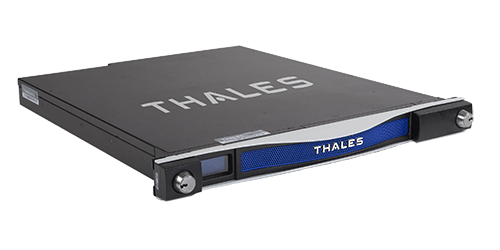
\includegraphics[width=0.4\textwidth]{figures/hsm-server.png}
                    \caption{An example of a HSM for installation in a server rack from Thales\footnotemark[1].}
                \end{figure}
                \begin{figure}
                    \centering
                    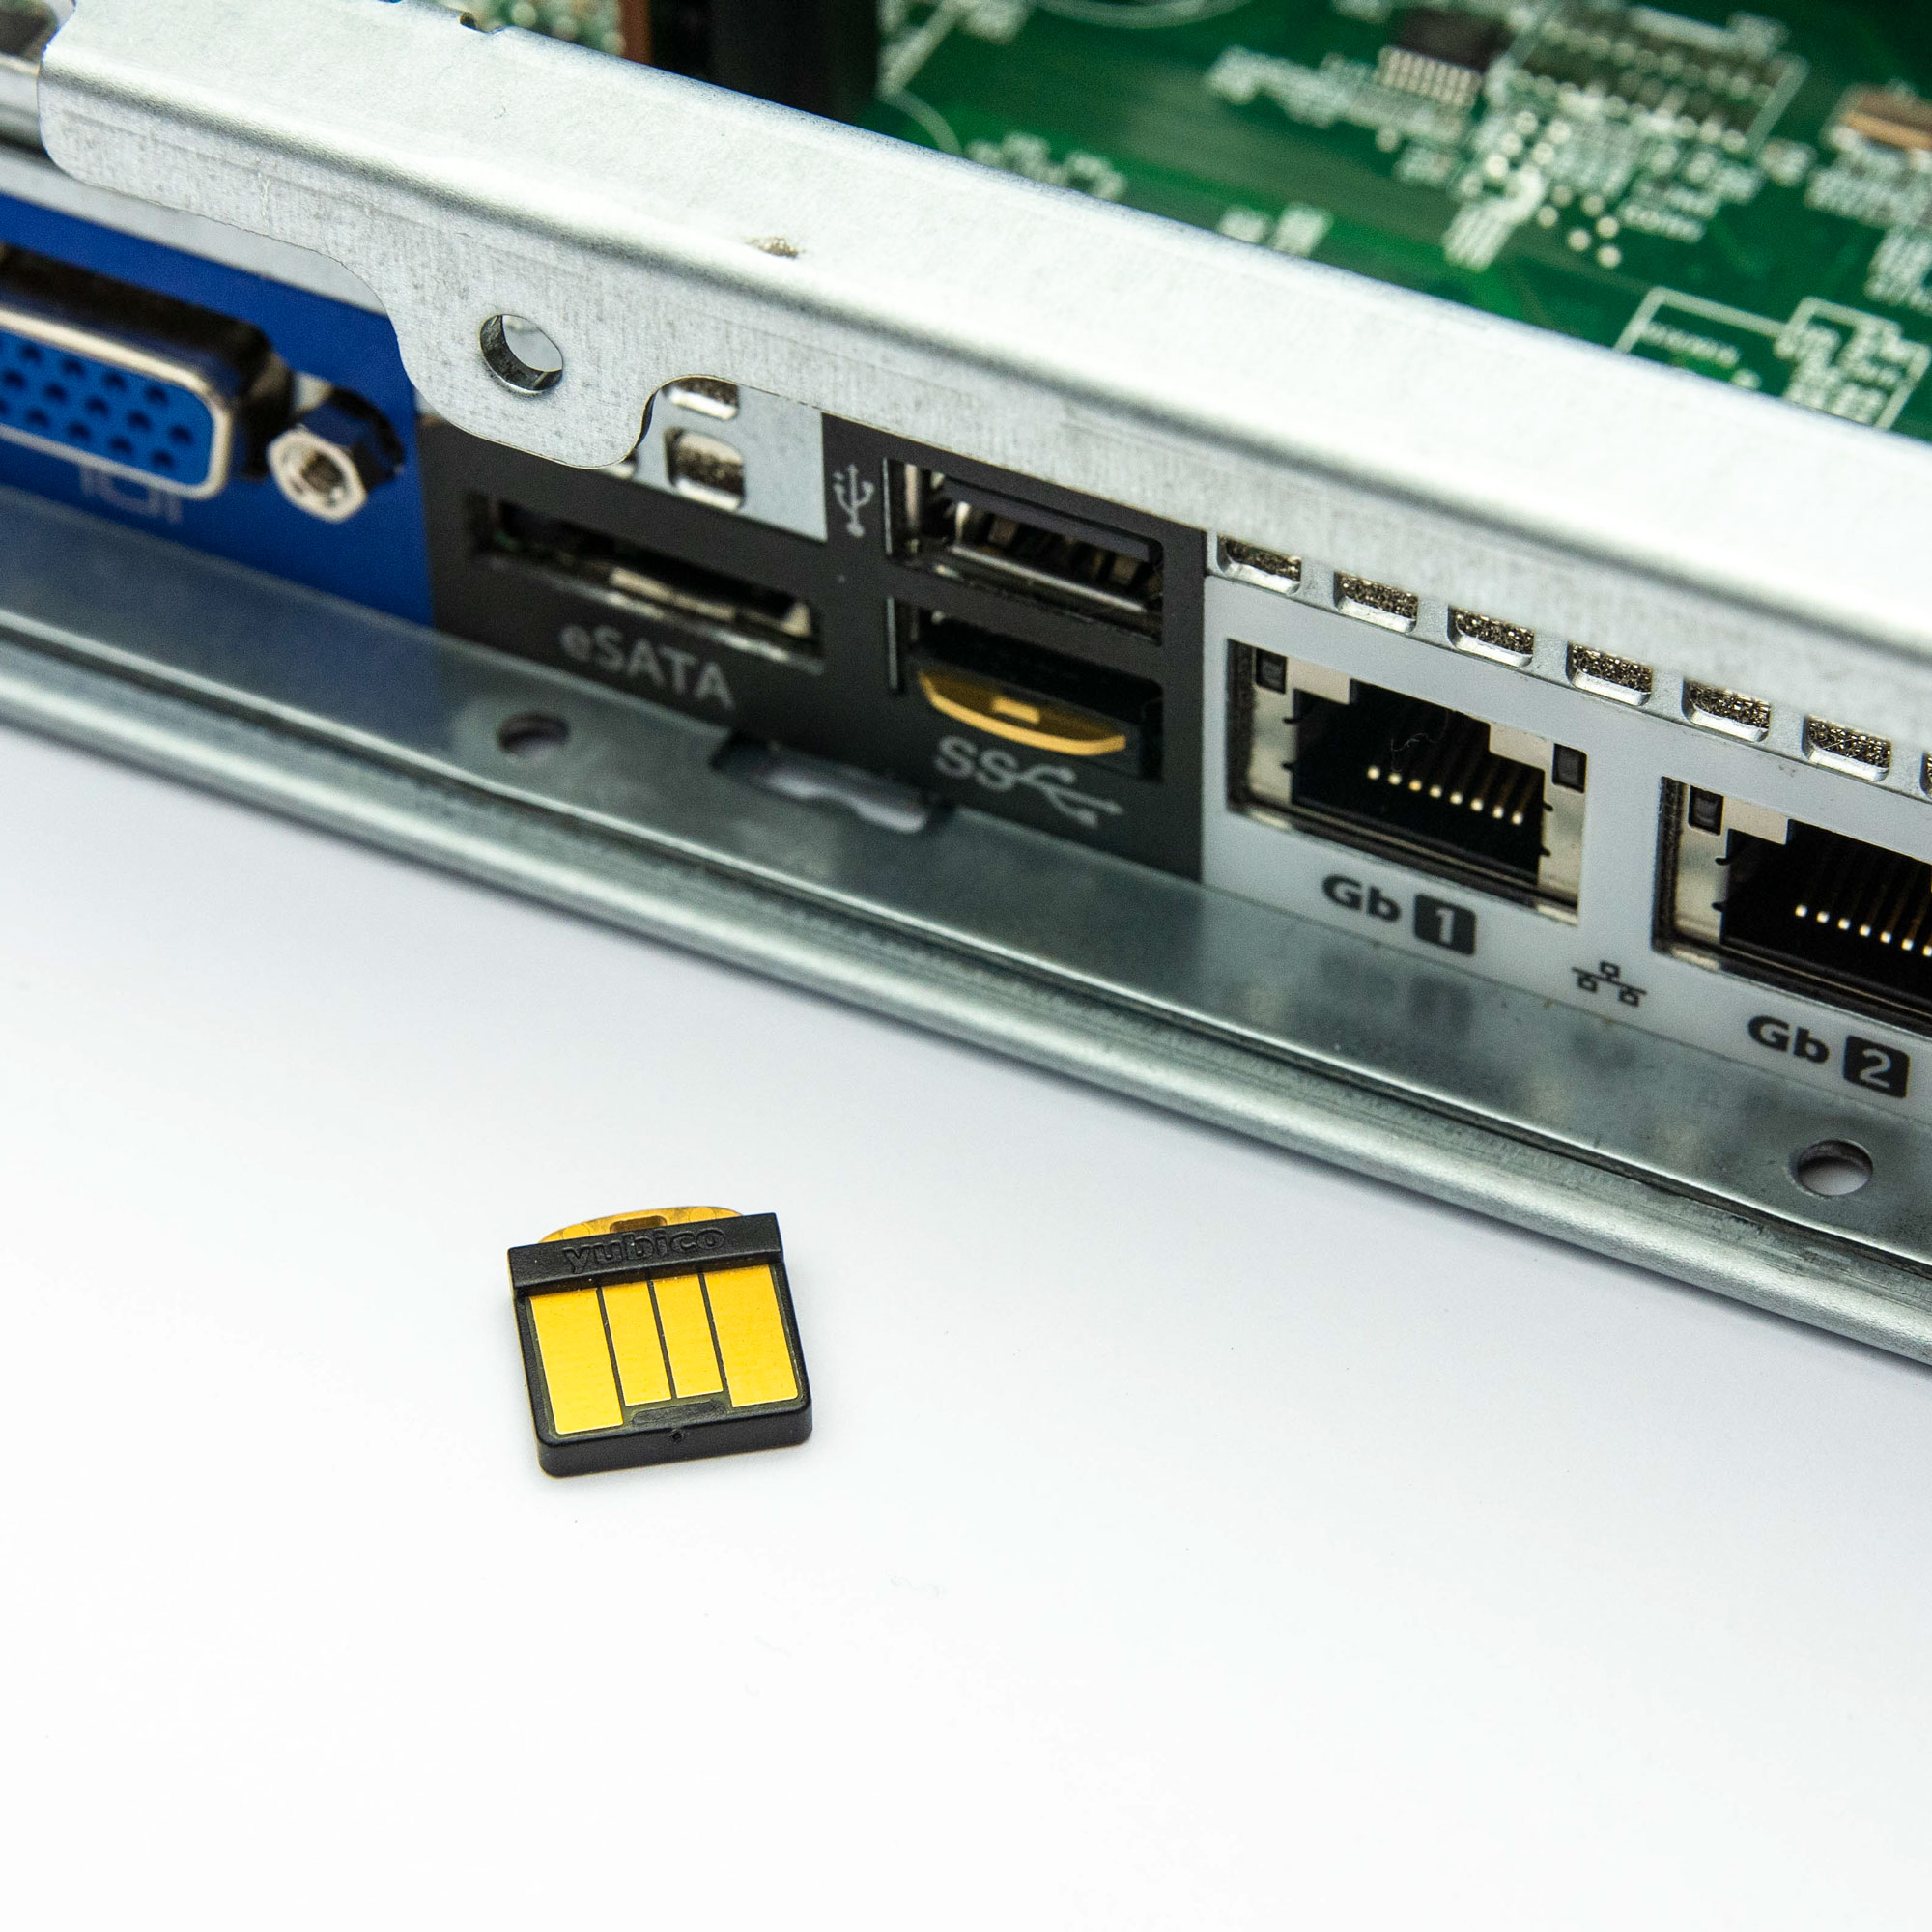
\includegraphics[width=0.3\textwidth]{figures/yubi-micro.jpg}
                    \caption{A very portable HSM from Yubico\footnotemark[2].}
                \end{figure}
            \end{block}




        \end{columns}
        \footnotetext{1: \fullcite{thales}}
        \footnotetext{2: \fullcite{yubi}}
\end{wide}
\end{frame}